%% sample template file for a MSc Thesis
%% The default is with two sided setup:
\documentclass[%
oneside,    %% uncomment for onesided layout
project,    %% uncomment not thesis but project report
nosummary   %% uncomment if no summary page should be generated
]{USN-MSc}

% The following command removes the chapter names form the header
% (comment/remove) if you prefer to have them:
\pagestyle{plain}

% --- Bibliography setup ---
%%% default is the "ieee" style
\usepackage[style=ieee, sorting=none]{biblatex}
%%% If you want to use "author-year" style
%%% where `\cite{Foo2011}` generates "Foo et al. (2011)"
%%% and   `\parencite{Foo2011}` generates "(Foo et al. 2011)"
%%% then comment the line above and use
%\usepackage[style=authoryear]{biblatex}
%%% or
%%% if you want to use "alphabetic" style then use
%%% where `cite[Foo2011]` generates "[Foo11]"
%%% then comment the line above and use
%\usepackage[style=alphabetic]{biblatex}
%%% instead.
%% load the bib file:
\addbibresource{MScThesis.bib}

\usepackage{lipsum} % just for providing fill text used in this template
\usepackage{array} % for adjusting tables?
\usepackage{pdflscape} % for landscape pages
\usepackage{longtable} % for tables spanning multiple pages

%These two are used to add frames to figures.
\usepackage{graphicx}
\usepackage[export]{adjustbox}

% --- general setup ---
%% Please fill in the following parameters:
\newcommand{\mytitle}{%
%% title:
Assignments for section 4 (W4.1-W4.5)
}

\newcommand{\mysubtitle}{%
%% master programme (for thesis only)
%% uncomment the appropriate one:
%%Electrical Power Engineering
%Energy and Environmental Technology
%Industrial IT and Automation
%Process Technology
}

\newcommand{\mykeywords}{%
%% keywords (for thesis only):
<keyword one, keyword two, \ldots>
}

\newcommand{\myauthor}{%
%% author(thesis) or group code (project):
223786 Lars Rikard Rådstoga
}

\newcommand{\myparticipants}{
%% group participants (for project only)
<First participant>\\
<Second participant>\\
<Third participant>\\
<Fourth participant>
}

\newcommand{\supervisor}{%
%% supervisor:
<Supervisor's Name>}

\begin{document}

% --- title page setup ---
%\USNtitlepage%
%%% Please provide the following information:
%%% #1 optional figure (set to {} if not wanted)
%{%
%  {\normalsize}
%  \begin{figure}[!ht]
%    \centering
%   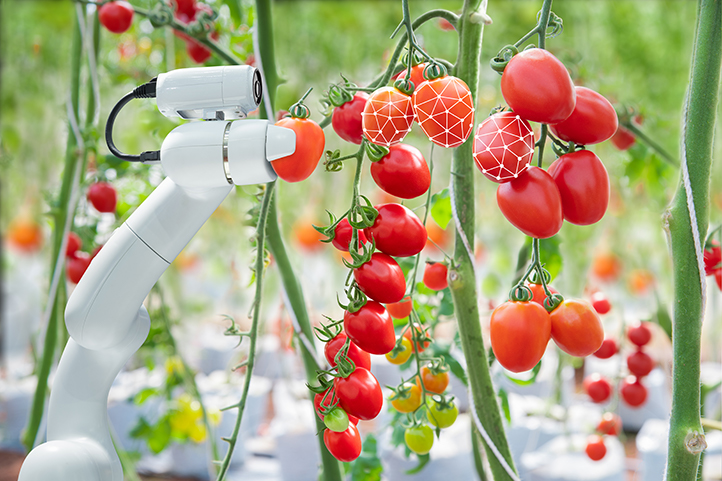
\includegraphics[width=0.8\textwidth]{TomatoPickerBot}
%   \label{fig:tomatoBot}
% \end{figure}
%}
% --- title page setup ---
\USNtitlepage%
%% Please provide the following information:
%% #1 optional figure (set to {} if not wanted)
{%
  {\normalsize}
  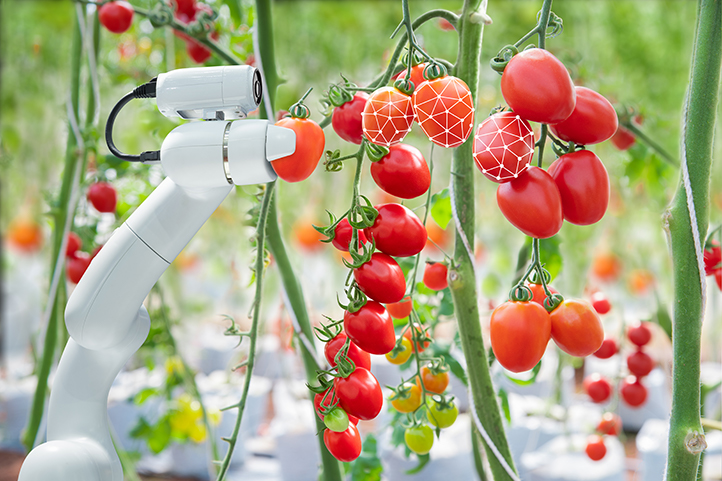
\includegraphics[width=\textwidth]{TomatoPickerBot}}
%% #2 Project partner:
{<Project partner>}
%% #3 Summary:
{%
  \lipsum[6-7]
}


%\chapter*{Preface}
%\label{ch:preface}
%\addcontentsline{toc}{chapter}{Preface}
%\lipsum[1-3]
%\bigskip
%Porsgrunn, \today

%\myauthor %% for thesis
%\myparticipants %% for project


%% table of contents
\tableofcontents
\addcontentsline{toc}{chapter}{\contentsname}

%\listoffigures % out-comment if unwanted
%\addcontentsline{toc}{section}{\listfigurename}

%\listoftables  % out-comment if unwanted
%\addcontentsline{toc}{section}{\listtablename}


\chapter{Capabilities}
\label{ch:cap}
This chapter contains a reflection of the capabilities of an autonomous system.
\section{Reflection}
To better understand the required capabilities of an autonomous system it is sensible to reflect upon the degree of automation required with respect to the four sliders of autonomy \cite{murphy2000introduction}, see figure \ref{fig:fourSliders}.

\begin{figure}[!ht]
  \centering
  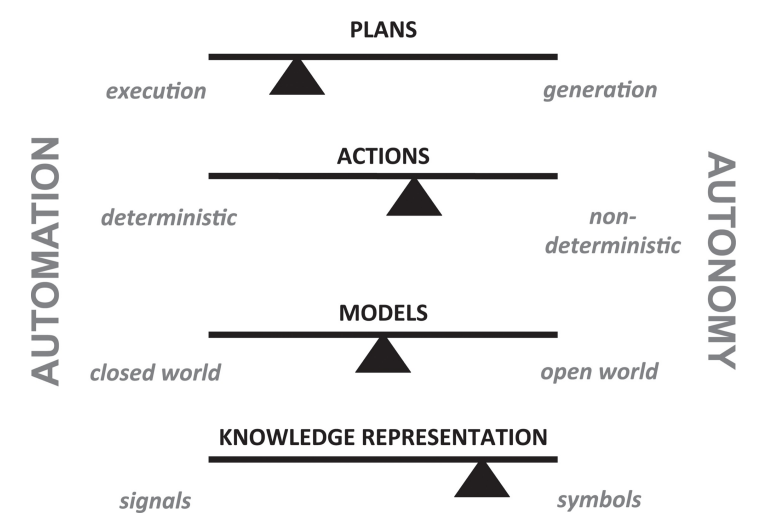
\includegraphics[width=0.80\textwidth, frame]{FourSlidersOfAutonomy}
  \caption{The four sliders of autonomy, an aid used to describe the degree of autonomy required for a system \cite{murphy2000introduction}.}
  \label{fig:fourSliders}
\end{figure}

The four sliders impact the degree of complexity of the system.
A higher degree of autonomy implies on-the-go planning, this means that a system could be able to adapt and prioritize tasks in order to minimize cost functions. It can perform big-picture planning by actively doing tasks such as coordinating with other actors, considering refueling timing, and more to minimize usage costs.

Autonomous systems' actions adapt to wear and tear or change in environment by using noisy sensors and closed-loop control algorithms. The more open and the less static the world is, more features need to take action like this. Some applications such as assembly in a factory will be operable with few or no sensory feedback, but robots like the Mars Rover will need a lot so it can operate cautiously.

The world model also impacts the degree of autonomy. In closed world examples, predictable environments such as a part of a factory, most of the world will be known a priori. In open world scenarios, however, the ground might be uneven or dirt can shift around. Objectives won't always appear in the same spots, etc. Open world models include less a priori information and more will be discovered a posteriori.

How knowledge is represented in the system is the last autonomy slider. In automated systems knowledge is mostly represented as signals such as GPS signals, sensory data and respective setpoints. E.g., to move from point A to B the automated robot would follow a coordinate-signal objective, but the autonomous robot would follow an order to move to fruit tree. This abstraction requires extra complexity.

\chapter{Frameworks}
\label{ch:frame}
This chapter contains a discussion on robotic frameworks.
\section{Discussion}

There are numerous frameworks and middleware options for robotics. Some options of which are dead projects, e.g. the Microsoft Robotics Studio, some are popular like the ROS framework, Gazebo, Rviz and Nvidia Isaac, and some might be under the radar like Hop. But the question is, do tools like these have what it takes to create intelligent AI based autonomous robots.

\begin{figure}[!ht]
  \centering
  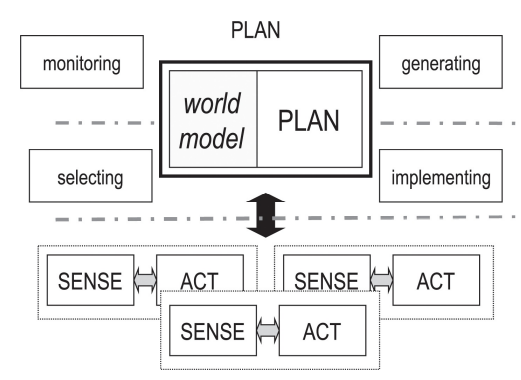
\includegraphics[width=0.80\textwidth, frame]{ReactiveAndDeliberativeLayers}
  \caption{The main functions within reactive and deliberative layers.}
  \label{fig:ReactDelib}
\end{figure}

As seen in figure \ref{fig:ReactDelib} an autonomous system can consist of multiple functions, these are often low coupled modules that require frameworks and/or middleware to work together. Such as ROS, the Robotic Operating System built upon Linux. Most importantly ROS includes infrastructure for communication between functions, this means that the ACT module can read information from the SENSE module in the reactive layer. ROS also comes with middleware that makes a lot of sensors and actuators work with minimal manual setup. Reactive layer functionality can then be created by fast-tracking sensory data to the ACT module where safety measures can be implemented, such as stop if unexpected obstacles appear. Deliberative layer functionality can then work asynchronously from the reactive. The deliberative layer can also subscribe to the sensory data and convert it to symbols that make up the world model. The four deliberative functions: generating, selecting, implementing, and monitoring can then able to work together to make intelligent decisions for the robot to achieve its goals.

\chapter{Industrial applications}
\label{ch:induApp}
This chapter contains a discussion regarding if and how autonomous systems can be used in industrial settings.
\section{Discussion}
Industrial plants today are already automated to a high degree and require operators to make reactive and preemptive measures to combat anomalies or unstable control. Automated systems take simple process inputs and regulating the process by minimizing the error to setpoints using algorithms such as PID to control actuators. This translates to the traditional sense, analyze, and act scheme depicted in gray in figure \ref{fig:Fig1Article1}. Instead, autonomous systems need to make more informed decisions, probably requiring data from multiple sources and the ability to make accurate predictions about future relevant developments in the relevant system.

\begin{figure}[!ht]
  \centering
  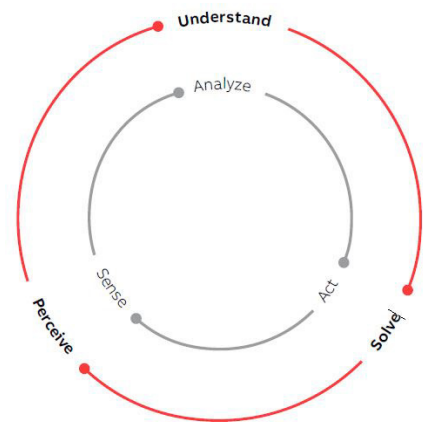
\includegraphics[width=0.50\textwidth, frame]{Fig1Article1}
  \caption{Loops in classical control systems (gray) and autonomous systems (red) \cite{GAMER2019454}}
  \label{fig:Fig1Article1}
\end{figure}

The scale between automation and autonomy is defined in different ways according to the field of study. Whether it is possible to implement autonomy to industrial settings depend on the definition of said scale. A definition of encapsulating categories of industrial systems can be seen in \ref{fig:Fig1Article2}. The automated system contains systematic process execution which can be as simple as hard coded arrays of coordinates and paths for a robot arm to follow. An intelligent automation system would in addition use sensory data to adapt to obstacles in the robot arms path, redirecting it. To truly reach autonomy the arm should also have self-governance and self-containedness. Self-governance meaning it should be able to do several high-level tasks like cooperating and decision-making without external help. Self-containedness is another branch of high-level tasks such as self-explanation and holistic affiliation, see figure \ref{fig:Tab3Article2} for explanations of some of these words.

\begin{figure}[!ht]
  \centering
  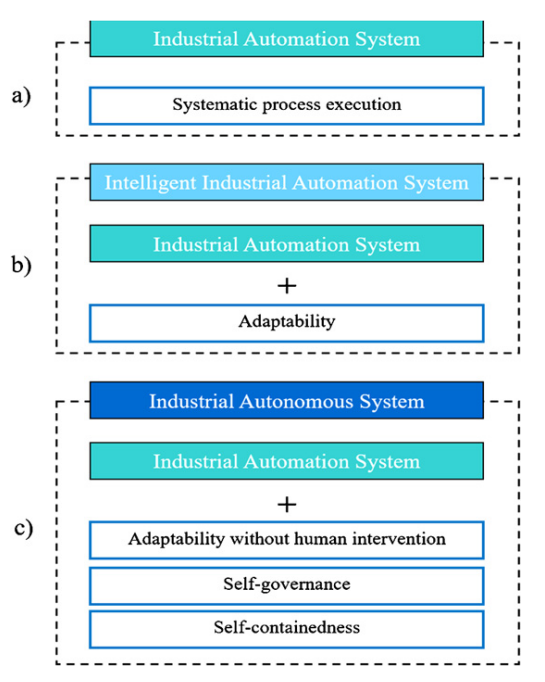
\includegraphics[width=0.50\textwidth, frame]{Figure1Article2}
  \caption{Differences between (classic) industrial automation systems, intelligent industrial automation systems, and industrial autonomous systems \cite{Müller}.}
  \label{fig:Fig1Article2}
\end{figure}


\begin{figure}[!ht]
  \centering
  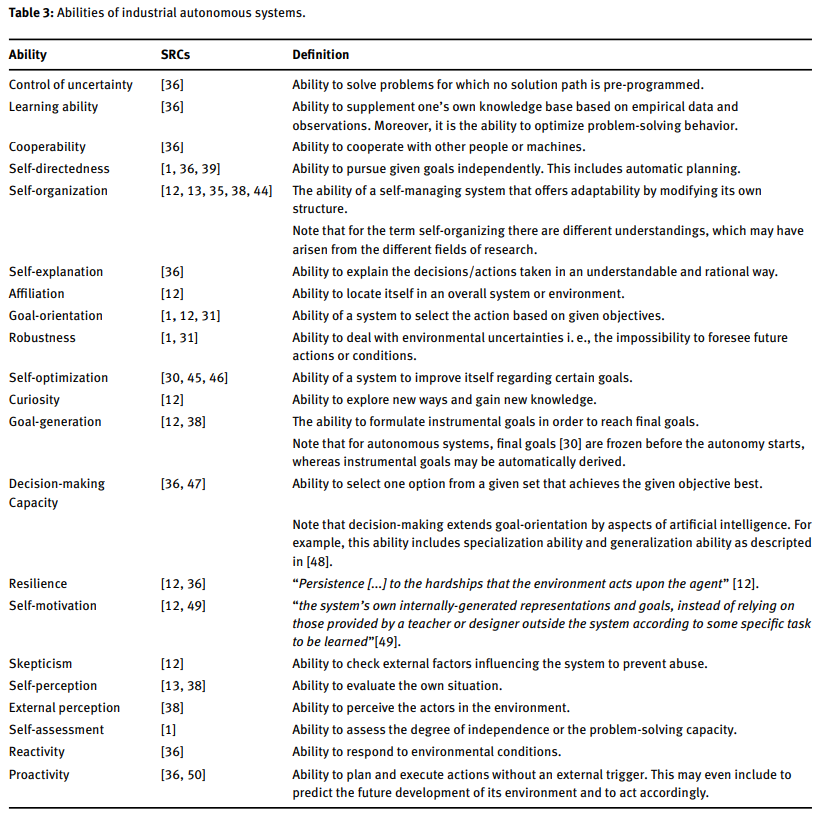
\includegraphics[width=0.90\textwidth, frame]{Table3Article2}
  \caption{Abilities of Industrial autonomous systems \cite{Müller}.}
  \label{fig:Tab3Article2}
\end{figure}



\chapter{Operational boundaries}
\label{ch:opBounds}
This chapter contains a definition of operational boundaries for the fruit-picker system.
\section{Definition}

Operational design domain (ODD) is a definition of a systems operational environment and complexity it needs to handle. This concerns the area, equipment, operations, and expected contribution from humans \cite{norwegiandefinitions}. The dynamic navigation task (DNT) is defined as the sum of all tasks needed to by the system and humans to handle all requirements set by the ODD \cite{norwegiandefinitions}. DNT is further split up into automatic tasks for the system to handle, operative exclusive tasks for humans to handle, and fallback tasks for safety in case situations outside the defined domain arises. Figure \ref{fig:OpBoundsEx} displays a visualization of this relationship.

\begin{figure}[!ht]
  \centering
  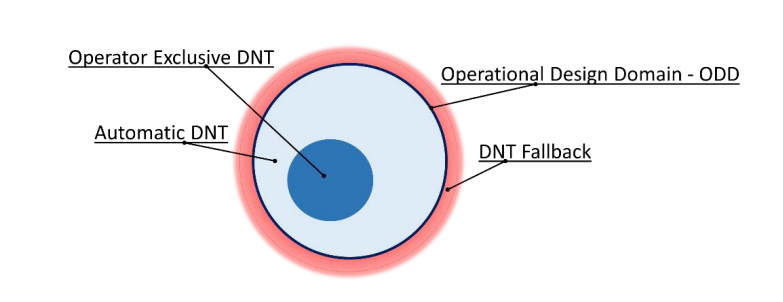
\includegraphics[width=0.80\textwidth, frame]{OperationalBoundsExample}
  \caption{Illustration of relationships between ODD, DNT and DNT Fallback \cite{norwegiandefinitions}.}
  \label{fig:OpBoundsEx}
\end{figure}

\section{Operational design domain}
The operational design domain for the fruit-picker robot should be an outdoor field in specifically geographically enclosed areas. The ground is often plastic or cloth around plants and the ground between them can be soil, hay, or bark. Fruit will grow on either bushes close to ground level or on trees. Any non-extreme weather conditions should be targeted. Farming is mainly not a winter activity, so it should be safe to target warmer weathers, i.e.: above 0℃.

Most tasks should be automatic, including: navigation between POIs, charging, loading/unloading collection baskets, fruit identification, fruit picking, anti-collision, interaction with other agents, operational condition reporting, data recording, actuator control, operations logging, and possibly more.

A handful of tasks should be carried out by human operators, such as: cleaning, maintenance, initialization, anomaly monitoring, and more.

Fallback procedures would be a few, but not limited to: safety stop, anti-theft lockdown, and reporting/signaling unexpected failure or damage.

\chapter{Overall capabilities of the fruit-picker system}
\label{ch:overalCap}
This chapter contains a description of all required capabilities: level of autonomy, main task description, HMI, and requirements for the robotic framework.
\section{Level of autonomy}

The level of autonomy required for the fruit-picker robot is generally high. The degree of autonomy might even be viewed as a piecewise function of time with the degree of autonomy varying between different tasks. Imagine the sliders in figure \ref{fig:fourSlidersFruit} changing from task to task and the figure displaying a potential average.

Planning capabilities of the system has to be generative to a high degree for most cases. This is because it will have tasks that will have varying solutions, every bush or tree will be different with fruit positioned differently, with variations in shape and color. It will be heavily reliant on sensory input which can be also be noisy from a multitude of reasons such as sensory, temporary disturbances like dirty equipment, changing environments, and more. So planning will need to be generative to adapt to lots of variations.

\begin{figure}[!ht]
  \centering
  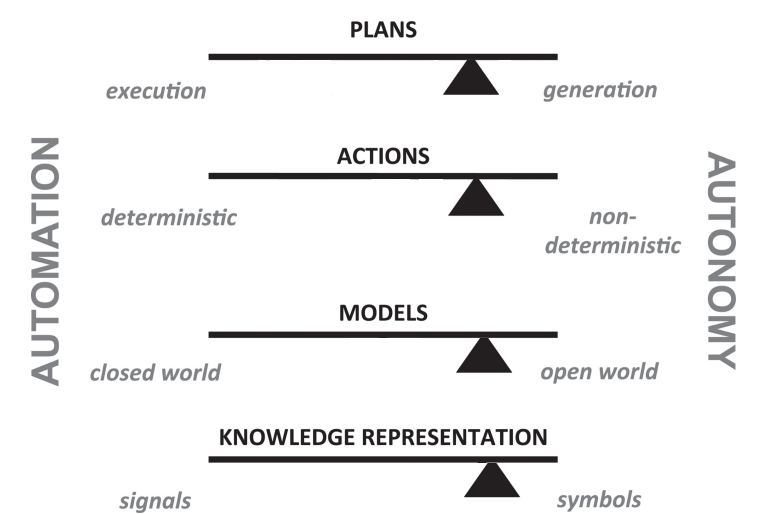
\includegraphics[width=0.80\textwidth, frame]{FourSlidersOfAutonomyFruitPicker}
  \caption{The four sliders of autonomy, reflecting degrees of autonomy required for the fruit-picker system \cite{murphy2000introduction}.}
  \label{fig:fourSlidersFruit}
\end{figure}

Actions will follow as mostly non-deterministic it will have to carry out tasks in an arguably stochastic world, will depend on noisy sensors and perhaps changing inner timings. The tasks such as identifying paths and obstacles, traversing them and similar with fruit picking will wary with every execution, starting points and goals will also never be truly equal.

World modelling will be performed with multiple layers. The boundaries of fields, defining the operational area will be static like in closed world models. However, within the closed world there will be both closed and open-world elements. The main outlines of plant and path locations will likely be useful initial information if it is easily available, but it should be hard to create properly. So for most things within the bounded world it will have to keep an open-world assumption. Boundary and coarse maps should be combined with LIDAR and camera data to aid the robot identify the open-world. So it should have some idea of where to move to find fruit, but know that things that move around and doesn't look like fruit might be something it should be careful of.

Knowledge should be converted to symbols in order to make the agent intelligent. This means that objectives, tasks and otherwise relevant items should be presented as abstractions or symbols. This means that it should have some idea of what it is doing.

\section{Description of main tasks}

The berry picker robot requires an array of capabilities in order to be satisfactorily autonomous. The table \ref{tab:breakdown} contains a list if main tasks broken down with sub-tasks involved in their respective tasks, this is meant to create a detailed functional overview of the system.


\begin{longtable}{| m{1.5cm} | m{3cm} | m{10cm} |}
  \caption{Main task breakdown.} \label{tab:breakdown}                                                                                                                                                                                        \\
  \hline
  Main-group
   & Sub-group
   & Description                                                                                                                                                                                                                              \\ \hline
  \multicolumn{3}{|l|}{1. High level planning}                                                                                                                                                                                                \\ \hline
  1.1
   & Meta planning
   & Use available information about the farm, to plan out where and when to harvest considering field geometry, ripeness estimations, harvesting efficiency of the robot and coordination with other units. This can be manually overridden. \\ \hline
  1.2
   & Macro planning
   & Keep track of what major task to do next, such as: relocating, harvesting, transporting, restocking and recharging.                                                                                                                      \\ \hline
  \multicolumn{3}{|l|}{2. Navigation and mapping}                                                                                                                                                                                             \\ \hline
  2.1
   & Identification
   & Use of sensors and vision systems to identify fruit trees/bushes, obstacles, fruit and more.                                                                                                                                             \\ \hline
  2.2
   & Navigation
   & Create a path by using installed map data, GPS signals, locally generated world view and tachometer and identified landmarks.                                                                                                            \\ \hline
  2.3
   & Maneuvering
   & Control the vehicle motor by speed and angular setpoints generated by the navigator, compensate for friction and steepness, react to unexpected sensory inputs and fail upwards to the navigator.                                        \\ \hline
  \multicolumn{3}{|l|}{3. Harvesting}                                                                                                                                                                                                         \\ \hline
  3.1
   & Identification
   & Use of sensors and vision systems to identify stems, fruit in terms of ripeness, damaged fruit, and more.                                                                                                                                \\ \hline
  3.2
   & Navigation
   & Every plant is different, so navigation tasks has different solutions for each fruit to be picked, identification is used to identify different parts of the plant in order to create a path for the robot arm.                          \\ \hline
  3.3
   & Maneuvering
   & Control the robot arm motor by speed and angular setpoints generated by the arm navigator react to unexpected sensory inputs or actuator performance, and fail upwards to the navigator.                                                 \\ \hline
  3.3
   & Sorting
   & The robot may be responsible for sorting and grading fruit based on ripeness and damage.                                                                                                                                                 \\ \hline
  \multicolumn{3}{|l|}{4. Monitoring}                                                                                                                                                                                                         \\ \hline
  4.1
   & Tracking
   & Check and record how the robot is operating compared to the planned tasks and calculated paths.                                                                                                                                          \\ \hline
  4.2
   & Reporting
   & Generate descriptions of what, how and why tasks are being executed.                                                                                                                                                                     \\ \hline
  4.3
   & Self diagnostics
   & Test and evaluate that sensors, actuators and other components are functioning correctly and accurately detecting and responding to stimuli.                                                                                             \\ \hline
  \multicolumn{3}{|l|}{5. Security}                                                                                                                                                                                                           \\ \hline
  5.1
   & Authorization
   & Accessing management software for updating, initializing, monitoring, and otherwise managing the robot will require both password and a two-factor authentication.                                                                       \\ \hline
  5.2
   & Geo-locking
   & Most robots will operate in statically definable areas, option to prohibit usage outside the designated area should be available.                                                                                                        \\ \hline
\end{longtable}

\section{Human-machine interaction}
The focus of the design of this autonomous fruit harvesting system is not on human-machine interaction in terms of overriding control. Instead, the goal of the system is to allow independent operation and make decisions without the need for human intervention.

The fruit harvesting robot should be designed to be self-sufficient and able to handle a wide range of tasks without the need for human input. This allows it to operate efficiently and effectively, and frees up humans to focus on other tasks that require their attention.

However, one of the key roles that humans play in the operation of autonomous harvesting robots is monitoring. These systems need to be closely monitored in order to ensure that they are functioning properly and achieving their intended objectives. This may involve monitoring the performance of the robots, checking for any potential issues, and making any necessary adjustments to ensure that they are operating efficiently.

In addition to monitoring, humans are also needed for the maintenance of autonomous harvesting robots. These systems require regular maintenance and servicing in order to continue functioning properly. This may involve tasks such as cleaning and lubricating the robots, checking and replacing worn parts, and performing any necessary repairs.

While autonomous harvesting robots are designed to operate independently, they still, for now, require human oversight and maintenance in order to function properly. Systems like these are important tools for improving efficiency and productivity in the agricultural industry, but they cannot operate without the support of human workers. Though, the aim is to improve independence in the future.

The human-machine interface for monitoring autonomous fruit harvesting robots should be designed to provide clear and intuitive information about the performance and status of the robots. This may include features such as:

\begin{itemize}
  \item Real-time visual displays of the robots' locations and movements, to help operators track their progress and identify any potential issues.

  \item Data displays and graphs showing the robots' performance metrics, such as the amount of fruit harvested, the speed at which they are operating, and any potential issues they are encountering.

  \item Alerts and notifications that inform operators of any potential issues or problems with the robots, such as low battery levels or mechanical problems.

  \item Control and configuration options that allow operators to adjust the settings and behavior of the robots, such as their speed, the amount of fruit they are allowed to pick, and where to harvest.
\end{itemize}

Overall, the human-machine interface for monitoring autonomous fruit harvesting robots should provide clear and easy-to-understand information about the performance and status of the robots, as well as the ability to adjust their behavior as needed. This will help operators to effectively manage the robots and ensure that they are operating efficiently and effectively.

\section{Requirements for a robotic framework}
There are a lot of features that can be helpful with programming the autonomous harvesting system, some of them are:

\begin{itemize}
  \item Real-time perception and analysis of the environment, including the ability to process sensory information from cameras, LIDAR, and other sensors.
  \item Planning and decision-making capabilities, including the ability to generate and execute plans based on the information it receives from the environment.
  \item Physical manipulation and control capabilities, including the ability to control the movement and actions of the robot.
  \item Adaptability and learning capabilities, including the ability to improve performance over time based on experience.
  \item Support for multiple programming languages, to allow users to write code in the language of their choice.
  \item A user-friendly interface that makes it easy for users to interact with the framework and create and debug their programs.
  \item Built-in tools for debugging and testing, to help users identify and fix any problems with their code.
  \item A library of pre-built functions and modules that can be used to quickly and easily add common functionality to a program.
  \item Support for distributed computing, to allow multiple robots to work together and share information and resources.
  \item Integration with external tools and services, such as simulation environments and cloud-based services.
  \item Support for safety and security, including features that help to prevent accidents and protect against malicious attacks.
\end{itemize}

Overall, a robotic programming framework should include a wide range of features to support the development of complex and powerful robotic systems. It should provide tools for real-time perception and decision-making, physical manipulation and control, and adaptability and learning, as well as a user-friendly interface and support for multiple programming languages and external tools and services.




















Overall, a robotic programming framework should include a wide range of features to support the development of complex and powerful robotic systems. It should provide tools for real-time perception and decision-making, physical manipulation and control, and adaptability and learning, as well as a user-friendly interface and support for multiple programming languages and external tools and services.


% A dummy command that causes all bibliographyentries to be displayed
% even though there were not cited in the document. Used for demonstration
% purposes only in this template file.
~\nocite{*}

\cleardoublepage

% The bibliography should be displayed here...
%\printbibliography[heading=bibintoc]
% You rather like to call the bibliography "References"? Then use this instead:
\printbibliography[heading=bibintoc, title={References}]


%\appendix
%\renewcommand{\appendixname}{Paper} %% So we get 'Paper X' displayed instead


%\chapter[Short Title of Paper A]{Title of Paper A (probably very long and therefore not good to have in the header)}
%\label{paper-a}
%
%\paragraph{Note}
%Since some papers tend to have a rather long title it is good to provide the optional short title which then will be displayed in the table of contents and header instead of the long original title.
%On the openening page of the chapter the orginal \emph{long} title will be displayed.\bigskip
%
%\emph{Short descriptive text of paper follows here.}\bigskip
%
%The paper itself needs to be included in the published form as PDF on the next pages.
%This can be done using the \texttt{pdfpages} package by adding the command:
%
%\begin{verbatim}
%\includepdf{pages=-,openright}{Filename}
%\end{verbatim}
%
%You can omit the \texttt{.pdf} when specifying the \texttt{Filename}. Also you should include always include the option \texttt{openright} since it would look strange to have the paper starting at the back of the cover page.
%
%There are more options like only adding specific pages:
%\begin{verbatim}
%\includepdf{pages=2-6,openright}{Filename.pdf}
%\end{verbatim}

%For more options see Appendix~\ref{paper-b} where the most important pages of the \texttt{pdfpages} manual were inlcuded using \texttt{pdfpages}.


%%% Command to include a PDF file directly including all pages:


%\chapter[Short Title of Paper B]{Title of Paper B}
%\label{paper-b}
%Short descriptive text of paper follows here.
%
%Here we included the first five pages of the \texttt{pdfpages} manual itself.
%
%\includepdf[pages=1-5,openright]{fig/pdfpages}
%
\end{document}

%%% Local Variables:
%%% mode: latex
%%% TeX-master: t
%%% End:
